% IEEE standard conference template; to be used with:
%   spconf.sty  - LaTeX style file, and
%   IEEEbib.bst - IEEE bibliography style file.
% --------------------------------------------------------------------------

\documentclass[letterpaper]{article}
\usepackage{spconf,amsmath,amssymb,graphicx}
\usepackage{graphicx}
\usepackage{tabularx}
\usepackage[export]{adjustbox}


% Example definitions.
% --------------------
% nice symbols for real and complex numbers
\newcommand{\R}[0]{\mathbb{R}}
\newcommand{\C}[0]{\mathbb{C}}

% bold paragraph titles
\newcommand{\mypar}[1]{{\bf #1.}}

% Title.
% ------
\title{Parallel SAT Solving}
%
% Single address.
% ---------------
\name{Jan Eberhardt, Jakub Lichman}
\address{Department of Computer Science\\ ETH Zurich\\Zurich, Switzerland}

% For example:
% ------------
%\address{School\\
%		 Department\\
%		 Address}
%
% Two addresses (uncomment and modify for two-address case).
% ----------------------------------------------------------
%\twoauthors
%  {A. Author-one, B. Author-two\sthanks{Thanks to XYZ agency for funding.}}
%		 {School A-B\\
%		 Department A-B\\
%		 Address A-B}
%  {C. Author-three, D. Author-four\sthanks{The fourth author performed the work
%		 while at ...}}
%		 {School C-D\\
%		 Department C-D\\
%		 Address C-D}
%

\begin{document}
%\ninept
%
\maketitle
%

\begin{abstract}
Satisfiability solving is an interesting problem with various applications.
In this report we describe how we implemented and parallelized a simple SAT solver.
We compare different parallelization variations and analyze their respective trade offs.
We achieved linear or even super linear speedups until up to 28 CPU cores compared to our sequential implementation.
\end{abstract}

\section{Introduction}\label{sec:intro}

\mypar{Motivation}
The boolean satisfiability problem (SAT) belongs to the most important problems in program analysis, verification and other disciplines of theoretical computer science.
It is used in the background of many applications, especially ones in the field of automated planning and scheduling, model checking (formal verification) and theorem proving.
The last decade brought many improvements to the SAT solving world in the form of advanced heuristics, pre-processing and processing techniques, and data structures that allow efficient implementation of search space pruning.
The past 10 years were also rich in improvements in parallelism.
Current trends in computer hardware design decreased performance per processing unit and pack more units on a single processor.
However, algorithms such as DPLL and CDCL were invented before the wide use of parallelism and therefore designed for sequential execution.
Since the SAT problem is NP-complete, we consider it a good candidate to be parallelized.

In our approach, we are trying to speed up SAT solving by running it on multiple cores with different techniques of search space partitioning.

The remainder of this report is structured as follows:
In the next subsection we provide some related work.
In Section \ref{sec:background} we introduce some core SAT concepts.
In Section \ref{sec:parallel_dpll} we explain how we parallelized DPLL.
In Section \ref{sec:exp} we show our experimental evaluation.
In Sections \ref{sec:discussion}, \ref{sec:futureWork} and \ref{sec:conclusion} we talk about some things we tried that did not work out, about possible extensions to our work and finally conclude.

\iffalse
The final comparison is done between different parallel versions and the sequential one.
The parallel versions are based on the DPLL algorithm, but we also investigated in a DPLL and CDCL in combination.
All algorithms can run on a theoretically unlimited number of CPU cores, but some scale better than others.
\fi

\iffalse
Experiments were run on a cluster where we were allowed to use at most 48 cores.
//TODO I think we can just leave this away.
Tests were taken from SATLIB - The Satisfiability Library \cite{cnf_website} and some were also created by our own random generator of formulas.
Our results show nice speedups of the parallel versions against the sequential one.
However, the parallel DPLL algorithm is still not able to outperform sequential CDCL.
//TODO I think we can just leave this away.
It shows how good CDCL actually is in comparison with DPLL.
\fi

\mypar{Related work}
Tomas Balyo et al. proposed the "HordeSat" solver, which can run on up to 1024 cores and is based on the CDCL algorithm.
Their parallel approach is different from ours, because it is portfolio based but with signs of search space partitioning. \cite{hordesat}

Most of the previous SAT solvers designed for computer clusters or grids use explicit search space partitioning.
Examples of such solvers are GridSAT \cite{gridsat}, PMSAT \cite{pmsat} or ManySat \cite{manysat}.

Jurkowiak et al. proposed a work stealing implementation for dynamic load-balancing. \cite{stealing}
Our work stealing approach is similar to what they proposed.

Berger et al. parallelized DPLL in Haskell. \cite{dpll_haskell}
Our DPLL search space partitioning is similar to what they proposed, but our solver is not limited to one machine and we can run on multiple compute nodes.

\section{Background}\label{sec:background}

\mypar{CNF}
A \textit{boolean variable} is a variable that can be assigned either to \textit{true} or \textit{false}.
A \textit{literal} of a boolean variable $x$ is considered to be in positive $x$ or negative  $\overline{x}$ form.
A \textit{clause} is then disjunction (OR) of literals.
A \textit{conjunctive normal form} (CNF) formula is a conjunction of such clauses.
Every propositional logic formula can be transformed to a CNF format.
For the sake of this report we assume that the formula is already in the CNF format.
However a transformation would be simple and straight forward based on basic propositional logic equivalence rules.

\iffalse
//TODO I think we can just leave this away.
However, measuring difficulty of CNF by these two factors is very inaccurate.
\fi

\mypar{SAT Solver}
A SAT solver is a program that is able to decide whether given formula is satisfiable.
More formally, a given formula $F$ is satisfiable \textit{iff} there \textit{exists} an assignment of literals $\theta$ that makes whole formula (\textit{CNF}) true.
Such a formula $F$ is then called \textit{satisfiable}.
If there does not exits such an assignment, the formula is \textit{unsatisfiable}.
Furthermore, a SAT solver should be able to provide a valid variable assignment in the \textit{satisfiable} case.

\mypar{History}
The first SAT solving algorithm was develop in 1960 by Martin Davis and Hilary Putnam \cite{dp}.
They used a resolution-based decision procedure.
Since the Davis-Putnam (or DP) algorithm was able to handle just valid formulas, a more general approach for SAT solving was needed.
//TODO: background check! I think DP can easily be extended to also handle unsat cases if I remember correctly...

In 1962 Davis, Putnam, Logemann and Loveland developed an extension of the DP algorithm, the DPLL algorithm.
DPLL is a backtracking-based search algorithm that still forms the basis for many extensions and efficient implementations of SAT solvers.
\begin{figure}
	\centering
	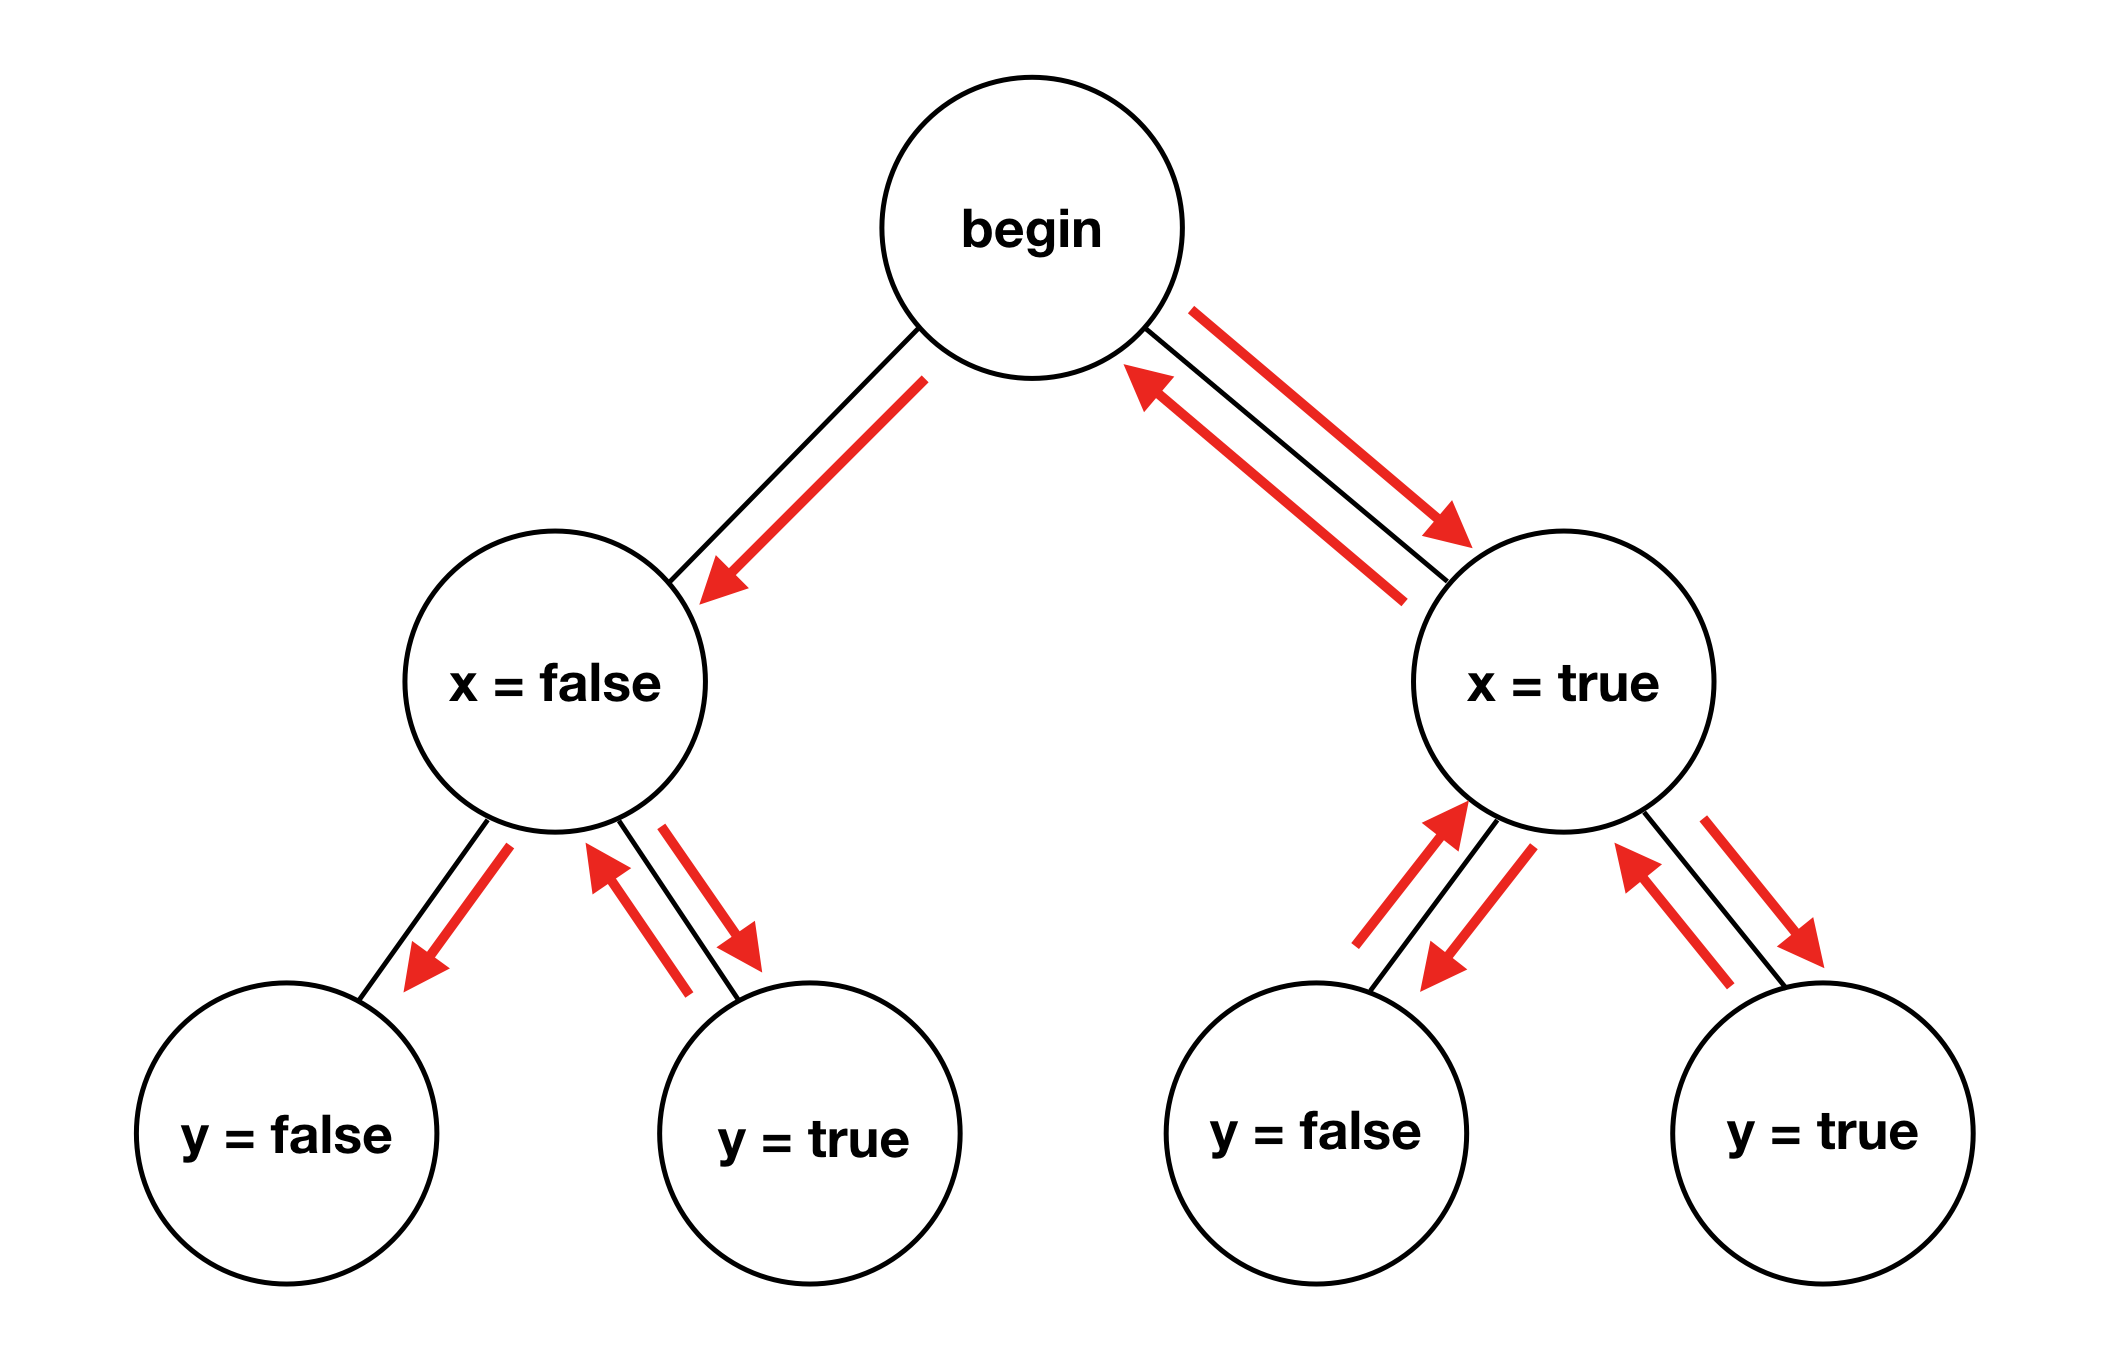
\includegraphics[width=\columnwidth]{figures/dpll-branching}
	\caption{The way how DPLL explores search space of CNF with two variables \textit{x} and \textit{y}.
		\label{fig:dpll-branching}}
\end{figure}

\mypar{DPLL}
DPLL solves a SAT problem by modelling it as a decision tree, variables can either be assigned to \textit{true} or \textit{false}.
In every step DPLL tries to find variables that are "automatically" assigned because of a previous decision,
if there are none it will pick a variable $v_i$ and assume a value for it.
If it later turns out that this decision was wrong it backtracks to that point and picks the negated assignment for variable $v_i$.
Figure 1 shows how DPLL's decision tree could look like for a simple formula with 2 variables.

\mypar{CDCL}
The algorithm performs as well as DPLL a depth-first search of the space of partial truth assignments.
In addition to DPLL, Conflict-Driven Clause Learning (\textit{CDCL}) adopts a pruning technique called learning.
While in DPLL it can happen that the same clause is solved multiple times, CDCL remembers them and in the next encounter avoids them.
More formally, learning extracts and memorizes information from the previously searched space to prune the search for future branches \cite{cdcl}.
Learning is done by adding clauses to the existing clause set.
Clauses are analyzed and stored whenever the search reaches a conflict state.
If it cannot be resolved by backtracking then the formula is unsatisfiable.
If all the variables are assigned and no conflict happened, then the formula is satisfiable.

\section{Parallelizing DPLL}\label{sec:parallel_dpll}

DPLL is a simple backtracking algorithm that explores the search space without any advanced techniques like learning and pruning.
As a result of this, it does not require any transfer of information between stages of solving and therefore it can be nicely parallelized.
The parallelization is not trivial, but far easier than in the case of CDCL, where in addition to load balancing we need to deal with sharing the learned clauses.

%We decided to parallelize DPLL because it is a relatively simple backtracking algorithm and therefore it does not require any advanced communication. Subtasks can be solved individually and therefore also on different nodes.

\mypar{DPLL Branches}
As shown in Figure \ref{fig:dpll-branching} the DPLL algorithm explores the search space with depth first search.
It does that as follows: If there are no more variables that can be assigned trivially, one variable is assumed to be either \textit{true} or \textit{false}.
That is exactly the point where we can do so called DPLL branching: continue on one branch and let some other node/processor solve the other branch.
We can call this point a branching point and it represents one node (or decision) in the DPLL decision tree.

In our work we considered two approaches to load balancing.
The first one is a master worker communication model, where one node, called \textit{master}, is in charge of storing partial models and passing them to \textit{workers} that will solve them.
The second approach is a work stealing communication model, where each node (or \textit{worker}) runs on its own and all \textit{workers} are equal.
If some \textit{worker} runs out of work and the formula is not solved yet, it picks a random other \textit{worker} and tries to steal a partial model from it, such that it can continue doing some work.

\mypar{Master Worker Model}
First we decided to design and implement the master worker model.
We considered this model to be the easiest to implement and therefore we picked it first.
The biggest challenge in parallelizing DPLL is load balancing.
The work cannot be split equally between workers at the beginning, because it would require knowledge of the depth of each branch.
This information cannot be inferred from a formula without solving it.
We want to avoid situations where work is not divided equally because we want to fully exploit the computing power of all nodes.

The \textit{master} is one of the \textit{n} available nodes and the other \textit{n-1} nodes are \textit{workers}.
At the beginning all workers are marked as free.
The \textit{master} starts solving by passing an empty model to the first free worker.
Each worker in every branching point takes one branch and sends the other branch as a partial model to the master.
When the master receives a partial model, it checks whether there exists some free worker.
If not it stores the model into its local stack.
Otherwise it sends it to a worker, which finished solving a branch with \textit{unsat} and therefore is free and needs more work.
This procedure is repeated until some worker finds a \textit{sat} model and sends it to the master.
The master then outputs the model and stops all workers.
If no worker found a \textit{sat} model, the master has an empty stack and all workers are free, then we know that the formula is \textit{unsat}.

While the master worker model is easy to understand and implement, it comes with several drawbacks.
The first of them is the lack of one node.
In the master worker model, one node (the master) is only used as a manager and therefore this node is not actually doing any computation.
The next issue is related to scaling.
The master can become a bottleneck with a certain number of nodes, because there is too much communication it needs to process and therefore workers need to wait longer for getting new partial models.
The last problem is also related to the amount of communication in this model.
Partial models and meta data are transferred every time a worker branches or wants to get a new partial model.
This communication could be reduced.
There is also communication at the beginning and at the end but this communication is necessary to distribute some initial work and stop all workers.

\mypar{Work Stealing Model}
Because of the drawbacks mentioned above we have decided to reduce and decentralize the communication by implementing a work stealing model.
The model treats all nodes \textit{equally} and therefore there is \textit{no master}, just workers.
All workers contain their own stacks with partial models to be processed.
This reduces the communication overhead because all produced models are stored locally instead of sending them to and storing them at the master.
However, the existence of this local stack breaks load balancing because some workers can work on bigger subtrees of the search space than the others.

Inequalities in load balancing are resolved by a mechanism called work stealing.
If some worker finished its work and no other worker has solved the formula yet, than it tries to "steal" a partial model from one of the other workers.
The process of stealing can be defined as follows:
A worker tries to steal from a randomly selected other worker until it finds a model or until someone else has found one.
There are two more phases in the communication model.
The first phase is the initial work distribution and the third one is the stopping criteria.
In the first phase worker 0 will take the role of the master and distribute starting models to all other workers.
Then all workers will try to solve their subtrees and in the case of running out of work they will try to steal work from some other worker (phase 2).
When some worker finds a \textit{sat} model, it will send it to worker 0, who stops all workers and outputs the final model (phase 3).
A master node is necessary at the end because there can be multiple workers that find a \textit{sat} model at the same time.
In our implementation, worker 0 prints the first obtained \textit{sat} model and ignores the others.

Our current work stealing implementation has one drawback:
It can only handle satisfiable formulas.
The stopping criteria in the unsatisfiable case was very trivial in the master worker model because there exists a moment when master's stack was empty and all workers were free.
In the work stealing model, no such a moment exits.
We do not have central node that controls the others and therefore knows in which stage each worker is.
We currently cannot detect if all workers are trying to steal (no worker has work left) and therefore we restrict ourselves just to satisfiable formulas with this communication model.

\mypar{Implementation}
We implemented both communication models in C++ with the help of MPI \cite{mpi}.
Our DPLL solver is implemented in C++ as well and therefore we can directly interact with MPI from within the solver.
We tried to keep the implementation of the DPLL algorithm and communication within nodes as separate as possible for better readability.
The implementation of parallel DPLL is straight forward and tries to follow good object oriented programming principles.
\iffalse
//TODO:
a) we did not use test driven development, we just had "some" end to end testing.
Test driven development would be if every interface method is tested for input output behavior and those test cases are written before the method body is implemented.
b) I'm not sure if terms as "information hiding" or "encapsulation" are relevant for this report.

We adapted test driven development with python wrapper that tests our program as black box.
We split program into classes with well defined interfaces according to their functions and applied proper encapsulation and information hiding.
\fi

We used \textit{vector}s from the C++ standard library to represent sets of clauses and sets of literals.
We used \textit{unsigned int}s as variable names, and \textit{boolean} types for sign and value of the literals and variables.
To implement the backtracking algorithm we used recursion, but we allocate all necessary data structures on the heap.
We did not experience any stack overflow issues.

\mypar{Correctness}
We tested our sequential DPLL solver on hundreds of formulas that we either randomly generated or took over from a SATLIB formula collection. \cite{cnf_website}
We ran each formula through z3 \cite{z3} and compared the result of z3 with our result.
The following cases have to be considered for each test case:
\begin{itemize}
    \item If both solvers return unsat, we pass the test case.
    \item If one solver returns sat and the other one unsat, we fail the test case.
    \item If both solvers return sat, we still need to check if the model our solver has returned is correct.
        To do that we can conjoin the model to the original formula and again run it through z3.
\end{itemize}

We ran both parallel implementations through the same set of formulas and checked correctness for each of them.
Assuming that our sequential implementation is correct, it is straight forward that our parallel implementation is correct as well:
we essentially solved the same set of sub problems but on different nodes and in a potentially different order.
The difference between the parallel and stealing version is just the load balancing and not in the searched space.
Both parallel versions solve the same partial models but they are distributed over the working nodes in a different way.

\section{Experimental Results}\label{sec:exp}
In this section we are going to present our experimental results for both versions of our parallel DPLL algorithm as well as their detailed description.

\mypar{Experimental Setup}
We ran both communication models on the Euler super compute cluster \cite{euler} on up to 48 cores, which was the maximum accessible number of cores to us, and requested 1 Gigabyte of memory per core. Euler contains 5 different types of nodes but each of them contains at least two 12-core Intel Xeon processors (2.5-3.7 GHz) and between 64 and 512 GB of DDR4 memory clocked at 1866, 2133 or 2666 MHz.

\mypar{Benchmark Formulas}
During our correctness testing and debugging phase of the core algorithm, we realized that random formulas generated by our own random formula generator are not suitable for performance testing.
Even if we picked formulas that contained the same amount of variables, clauses and literals per clause, we observed large variations in run time between them.
This is caused by the completely random structure of formulas generated by our generator.
Therefore we used a set of 14 formulas taken from a SATLIB formula collection as a benchmark set.
The set contains different real world problems modeled as a boolean formulas from various domains such as planning problems,
all-interval series encodings, flat graph coloring, inductive inference, etc.
Our benchmark set also contains a few random formulas that were taken from the SATLIB formula collection as well.
Table \ref{tab:benchmark_set} in the Appendix section contains a detailed listing of the used formulas together with their description.
For the coming subsections we reduced the set of benchmark formulas to a representable subset of size 6 for readability reasons.
We included the corresponding figures for the other 8 formulas in the Appendix section.

\mypar{Master Worker}
We compared the run times of the master worker communication pattern with the sequential version of DPLL.
The achieved speedup is shown in Figure \ref{fig:dpll_parallel_speedup}.
\begin{figure}
    \centering
    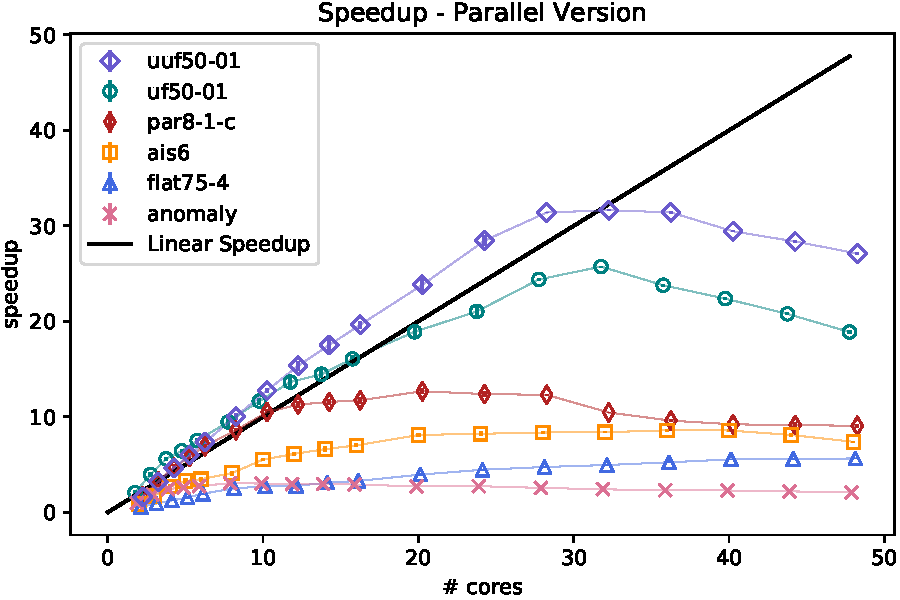
\includegraphics[width=\columnwidth]{figures/scaling_parallel_subset_dpll_scaling_tar.pdf}
    \caption{Average speedup of master worker parallel DPLL implementation compared to sequential DPLL.
    The 95\% confidence intervalls are shown as error bars but too small to be visible in some cases.
    \label{fig:dpll_parallel_speedup}}
\end{figure}
It can be inferred from the figure that the achieved speedup factor heavily depends on the formula.
But it is not just the "size" of the problem or time required to solve a formula with the sequential algorithm that influences the speedup factor.
As shown in Table \ref{tab:cnfs_representatives} the formulas where we reached the highest speedup are not necessarily the ones with the longest time to solve sequentially or the largest number of variables (highest upper bound on the depth of the decision tree).
Note that the best speedup in this subset is achieved for the randomly generated formula (uf50-01).
For the random formulas it is easy to explain why the speedup goes down with more than 32 cores.
It is caused by moments in the solving process when the master is no longer able to serve all the workers at the same time.
Therefore some workers have to wait longer to obtain the next partial model.
This problem starts to occur when the number of cores is larger than 30.
The overall average waiting time of all workers, shown in Figure \ref{fig:dpll_parallel_waiting}, shows this problem.
The waiting time is considered to be the time that some worker spends waiting for a new partial model from the master.
The overall waiting time is the sum of all waiting time periods of all workers, averaged over different runs of the same formula.
\begin{figure}
	\centering
	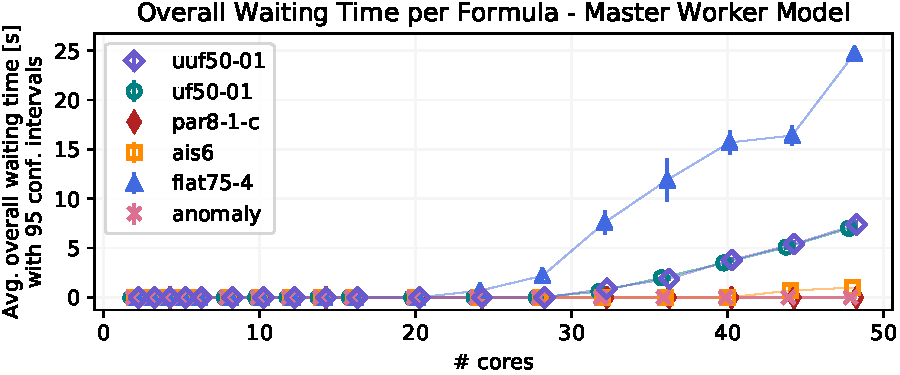
\includegraphics[width=\columnwidth]{figures/waiting_parallel_subset_dpll_scaling_tar.pdf}
	\caption{Average overall waiting time of workers per cnf in the parallel version.
		All waiting times per worker are summed up.
		The 95\% confidence interval are shown as error bars.}
	\label{fig:dpll_parallel_waiting}
\end{figure}

The cases where the speedup is not so significant are real world problems.
The structure of their decision trees is less random.
The small speedup is caused by the way the decision tree is traversed.
While the sequential implementation deterministically does a depth-first search and therefore gives us some ordering guarantees,
the parallel version sends all subbranches to the master and gives no ordering guarantees.
It might happen that a worker is "close" to a solution but then receives a partial model in a completely different part of the decision tree that might be unsatisfiable all together.
The size of the subtree where we will not find a solution depends on the structure of the formula.
This is also the explanation why we achieved super linear speedup in some other cases:
There we were lucky enough to reach the final solution with less iterations than in the sequential case.

\begin{table}
    \centering
    \begin{tabular}{|l|c|c|}
        \hline
        Formula & seq. runtime [ms] & \# vars/clauses \\
        \hline
        \hline
        uf50-01 (sat) & 7890.9 $\pm$ 44.31 & 50/218\\
        \hline
        par8-1-c (sat) & 2185.0 $\pm$ 32.88 & 64/254\\
        \hline
        ais6 (sat) &  2964.0 $\pm$ 41.54 & 61/581\\
        \hline
        flat75-4 (sat) & 26284.6 $\pm$ 172.65 & 225/840\\
        \hline
        anomaly (sat) & 279.7 $\pm$ 6.74 & 48/261\\
        \hline
        uuf50-01 (unsat) & 13404.2 $\pm$ 102.94 & 50/218\\
        \hline
    \end{tabular}
    \caption{Overview of benchmark subset formulas.}
    \label{tab:cnfs_representatives}
\end{table}

\begin{figure}
	\centering
	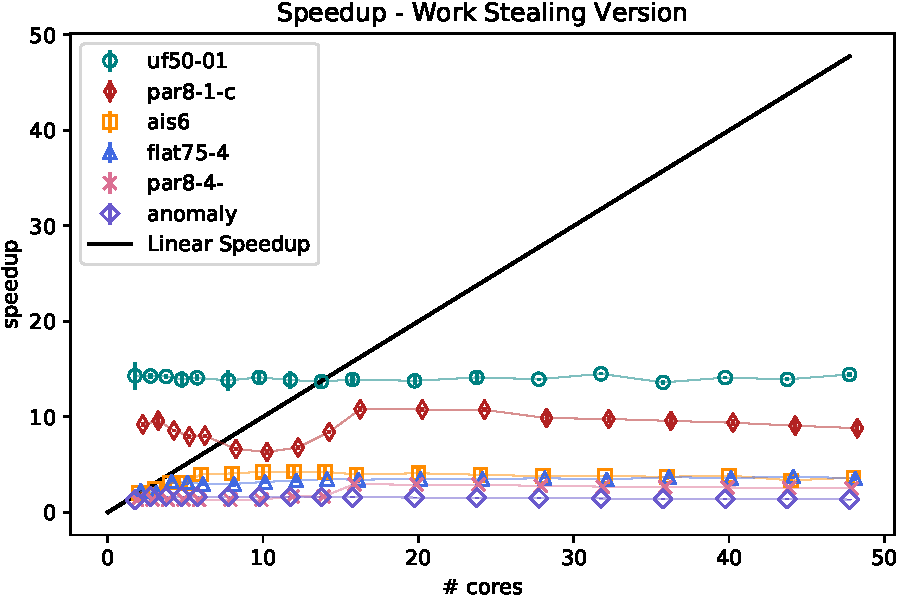
\includegraphics[width=\columnwidth]{figures/scaling_stealing_subset_dpll_scaling_tar.pdf}
	\caption{Speedup of work stealing parallel DPLL implementation compared to sequential DPLL.
		\label{fig:dpll_stealing_speedup}}
\end{figure}

\mypar{Work Stealing}
Similar to the previous comparison, we compared our parallel work stealing model to the sequential DPLL version.
The speedup that we achieved is shown in Figure \ref{fig:dpll_stealing_speedup}.
With the work stealing model we achieved large speedups for a small number of cores but essentially did not gain from adding more cores after some limit.
The reason for this is again the way how we traverse the decision tree.
In theory we should do something that is similar to a global breath first search and local (per node) depth first search in this model.
However because of phase 0 mentioned in Section \ref{sec:parallel_dpll}, the "global breath first" search part is not really a breath first search.
Each worker starts in a node in the decision tree that is one level shifted inwards from the right-most subbranch of the tree.
That means that if the formula is satisfiable, we are guaranteed that at least one worker is working on the correct subtree already after the first decision and will never solve models of the other subtree.
\iffalse
//TODO: not sure if this is required...
We do not have this guarantee for the master worker pattern because here workers jump out of their search space context every time they request new model from master.
It does not guarantee that model that worker receives is in the same context (subtree) as previous one.
Therefore it can easily happen that all workers are working on wrong subtree and they will move to the correct one just after finishing the wrong one.
\fi
As an result, we outperform master worker with the work stealing version with only a few cores.
But do not gain that much from adding more cores since the search space is split in a non-uniform way.

\mypar{Communication Overhead}
One of the reasons why we intorduced a work stealing mechanism was that it should drastically reduce the amount communication (bytes transferred) between cores.
Our experimental results prove that and they are shown in Figures [xxx] and [yyy].
From Figure [xxx] it can be inferred that the amount of communication rises with the number of cores in the master worker model.
In Figure [yyy] on the other hand the amount of communication does not increase that much with more cores.
//TODO: actually create those figures and verify that this is what's happening!
It is caused by reduced amount of partial model transfers, as mentioned in Section \ref{sec:parallel_dpll}.
However as we discussed in the previous subsection, the amount of communication is not the only limiting factor.
Master becoming the bottleneck when adding more cores is the main factor.
The measured waiting time per worker did not increase for the work stealing version as it did increase for the master worker model, which is shown in Figure \ref{fig:dpll_parallel_waiting}.

\section{Discussion}\label{sec:discussion}
In this section we are going to discuss some approaches that we tried during development but that did not work as expected or we had to stop investigating possible solutions because of time constraints.

\mypar{DPLL-CDCL Hybrid Parallel Solver}
We have implemented a fully working CDCL solver.
Its correctness was proven with the same testing infrastructure that we use to test our DPLL implementation.
The sequential version of the CDCL solver was faster than the sequential DPLL implementation for all of our benchmark formulas.
Quite naturally we tried to plug that solver in locally at the workers to boost the performance.
The way we did it is the following:
\begin{itemize}
    \item First we run DPLL in parallel (it does not matter which of the two communication patterns we pick) and we only branch a certain number of times per worker.
    \item After that "branching limit" is reached we switch to CDCL and solve the whole subtree of the original decision tree locally.
    \item When CDCL terminates, we either found a solution or get a new model (either from the master or another worker) and solve it again with CDCL.
\end{itemize}
This hybrid approach showed worse performance than we expected.
The reason for this is the following:
When running DPLL globally, we essentially create multiple smaller problems.
Smaller problems for the DPLL algorithm, which means they are easier and faster to solve than the original problem for a DPLL solver.
For the CDCL algorithm on the other hand those sub-problems are not necessary easier.
Some of those sub problems might actually be a lot harder than the original problem,
because with the made assumption by a DPLL decision step we could add a new conflict that was not there in the original problem.
As a result our hybrid parallel approach is slower than sequential CDCL in many cases.

We ran everything we discussed in Section \ref{sec:exp} with the hybrid parallel solver for different branching limits.
We do not include any further information in this report because of space limitations.
Overall the performance of this DPLL-CDCL hybrid solver was worse than both sequential CDCL and parallel DPLL with both of the two parallelization models.

\section{Future Work}\label{sec:futureWork}
In this section we are going to discuss possible extensions and improvements of our work.

\mypar{Improvements}
As presented in Section \ref{sec:exp} during the evaluation and measurements phase of our project we detected several drawbacks in our approach that could be improved.

First and the most important one is the decision tree traversal.
One would need to ensure a more uniform distribution of the search space among the workers for both models.
For instance we should avoid situations where one or no worker is working on the left part of the decision tree and all the other workers on the right part.

A second improvement would be to enhance the stealing effectiveness.
Stealing should no longer be completely random.
One could try to remember the stealing attempts and steal from workers that have the most partial models in their local stacks.

\mypar{Extensions}
Our current work stealing model implementation is only able to handle \textit{sat} formulas.
For handling \textit{unsat} formulas one would need to detect if all workers are trying to steal work.

Another interesting extension would be to fully parallelize the CDCL algorithm.
It would require sharing of learned clauses, which could be implemented by extending both of our communication models.

\section{Conclusion}\label{sec:conclusion}
SAT solving is after six decades of intensive research still a hot topic in theoretical computer science.
In our approach we tried to leverage more processor cores to get more computing power for solving SAT problems.
We parallelized the DPLL algorithm with two different communication models.
A master worker model with a central management node (the master) and a work stealing model where we try to reduce the communication overhead to a minimum.
Even though we identified deficiencies in both of our models we were still able to outperform our sequential DPLL implementation with both models.
For some formulas we were even able to outperform our sequential CDCL implementation.
We also investigated in a hybrid approach with global DPLL and local CDCL, which unfortunately did not bring the desired performance increase.

% References should be produced using the bibtex program from suitable
% BiBTeX files (here: bibl_conf). The IEEEbib.bst bibliography
% style file from IEEE produces unsorted bibliography list.
% -------------------------------------------------------------------------
\bibliographystyle{IEEEbib}
\bibliography{bibl_conf}

\newpage
\section{Appendix}
This section contains additional information that is not strictly part of the report.

\begin{table}[h]
    \centering
    \begin{tabularx}{\columnwidth}{|l|X|}
        \hline
        File names & Description\\
        \hline
        \hline
        anomaly, medium & SAT-encoded blocks world planning problems\\
        \hline
        ais6, ais8 & SAT-encoded All-Interval Series problems\\
        \hline
        flat50-1, flat75-4 \\ flat 75-8 & SAT-encoded "Flat" Graph coloring problems (J. Coberson's flat graph generator is used\\
        \hline
        ii8a1 & Inductive inference, stem from a formulation of boolean function synthesis problems\\
        \hline
        par8-1-c, par8-4- & Instances for learning the paritiy function\\
        \hline
        uf50-01, uf75-01 & Uniform random 3-sat, satisfiable\\
        \hline
        uuf50-01, uf50-02 & Uniform random 3-sat, unsatisfiable\\
        \hline
    \end{tabularx}
    \caption{Description of benchmark problems.}
    \label{tab:benchmark_set}
\end{table}

\begin{figure}[h]
    \centering
    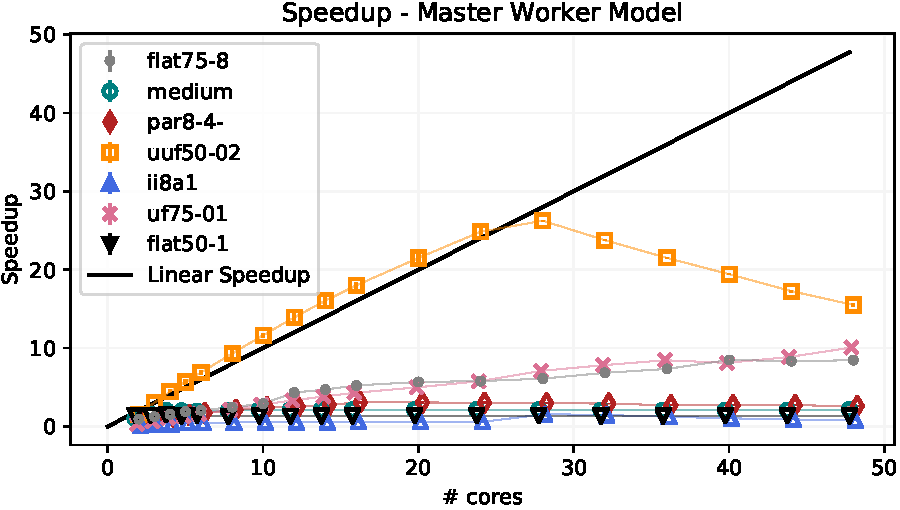
\includegraphics[width=\columnwidth]{figures/scaling_parallel_non_subset_dpll_scaling_tar.pdf}
    \caption{Average speedup of master worker parallel DPLL implementation compared to sequential DPLL.
    The 95\% confidence intervalls are shown as error bars but too small to be visible in some cases.
    Other subset.}
    \label{fig:dpll_parallel_speedup_non}
\end{figure}

\begin{figure}[h]
    \centering
    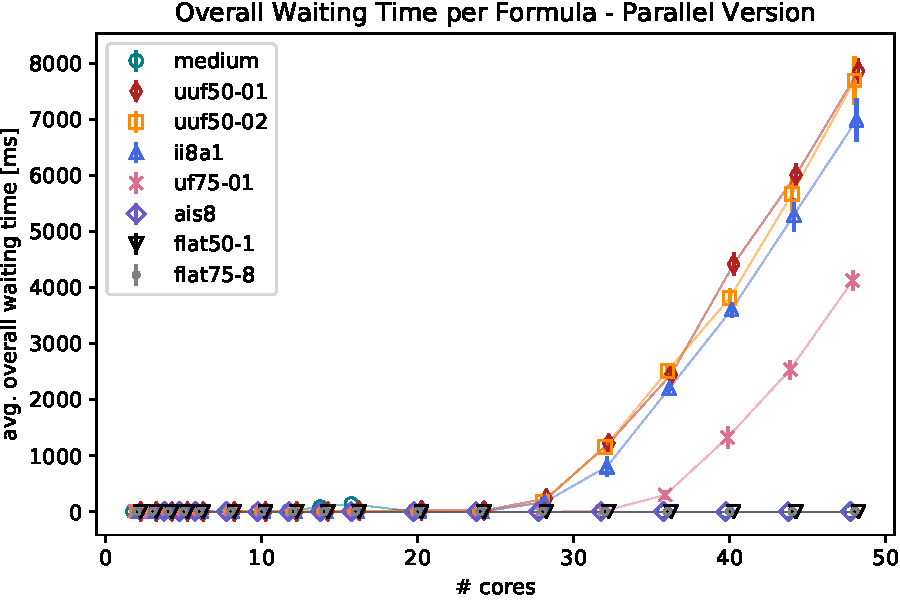
\includegraphics[width=\columnwidth]{figures/waiting_parallel_non_subset_dpll_scaling_tar.pdf}
    \caption{Average overall waiting time of workers per cnf in parallel version.
    All waiting times per worker are summed up.
    The 95\% confidence interval are shown as error bars.
    Other subset.}
    \label{fig:dpll_parallel_waiting_non}
\end{figure}

\begin{figure}[h]
    \centering
    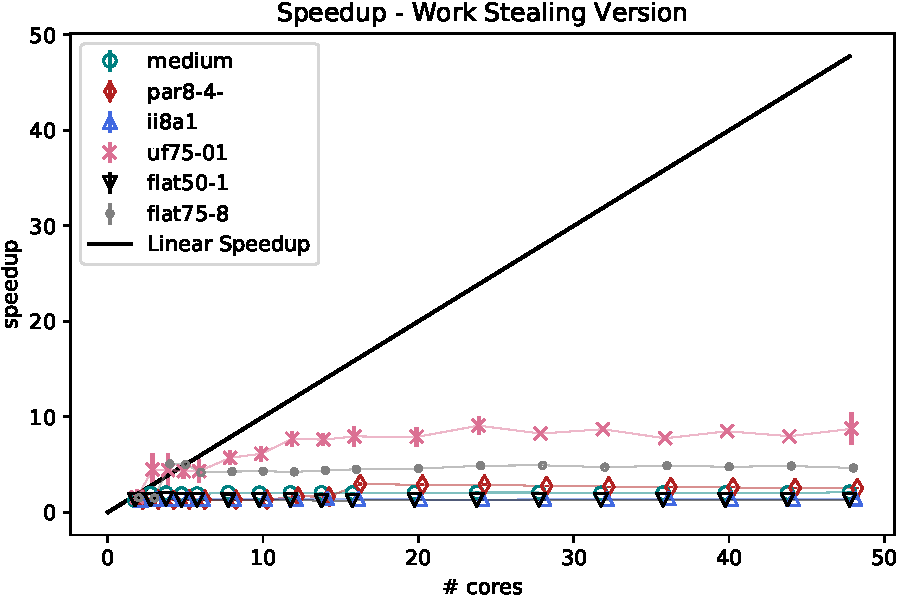
\includegraphics[width=\columnwidth]{figures/scaling_stealing_non_subset_dpll_scaling_tar.pdf}
    \caption{Speedup of work stealing parallel DPLL implementation compared to sequential DPLL.
    Other subset.}
    \label{fig:dpll_stealing_speedup_non}
\end{figure}

\begin{figure}[h]
    \centering
    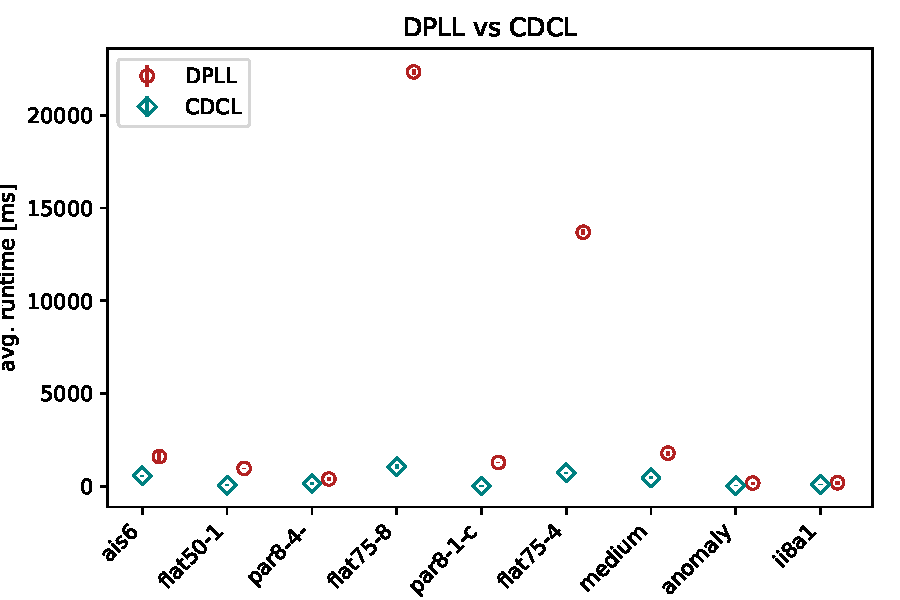
\includegraphics[width=\columnwidth]{figures/dpll_vs_cdcl.pdf}
    \caption{DPLL vs CDCL sequential runtime. Average runtime with 95\% confidence intervals.}
    \label{fig:dpll_stealing_speedup_non}
\end{figure}

\begin{table}
    \centering
    \begin{tabular}{|l|l|c|}
        \hline
        Formula & Best Solver Configuration & Runtime [ms]\\
        \hline
        \hline
        anomaly & CDCL sequential & 16.2 $\pm$ 4.18 \\
        \hline
        medium & CDCL sequential & 414.8 $\pm$ 32.94 \\
        \hline
        ais6 & DPLL master worker, 14 cores & 343.3 $\pm$ 3.58 \\
        \hline
        ais8 & DPLL master worker, 48 cores & 3015.3 $\pm$ 58.85 \\
        \hline
        flat50-1 & CDCL sequential & 36.4 $\pm$ 9.07 \\
        \hline
        flat75-4 & CDCL sequential & 702.8 $\pm$ 38.18 \\
        \hline
        flat75-8 & CDCL sequential & 1054.2 $\pm$ 50.72 \\
        \hline
        ii8a1 & DPLL master worker, 6 cores & 72.2 $\pm$ 0.79 \\
        \hline
        par8-1-c & CDCL sequential & 15.2 $\pm$ 2.28 \\
        \hline
        par8-4- & DPLL master salve, 2 cores & 132.2 $\pm$ 2.22 \\
        \hline
        uf50-01 & CDCL sequential & 31.5 $\pm$ 9.21 \\
        \hline
        uf75-01 & DPLL master worker, 32 nodes & 297.4 $\pm$ 7.99 \\
        \hline
        uuf50-01 & DPLL master worker 24 nodes & 187.5 $\pm$ 5.59 \\
        \hline
        uuf50-02 & DPLL master worker 24 nodes & 148.9 $\pm$ 2.85 \\
        \hline
    \end{tabular}
    \caption{Benchmark formulas with best performing configuration.}
    \label{tab:cnfs_parallel}
\end{table}


\end{document}

